\documentclass[11pt]{article}
\usepackage[T1]{fontenc}
\usepackage{lmodern}
\usepackage[margin=1in]{geometry}
\usepackage{amsmath,amssymb,amsthm,mathtools}
\usepackage{graphicx,booktabs,tabularx,array}
\usepackage{xcolor,microtype,enumitem,fancyhdr}
\usepackage[colorlinks=true,linkcolor=blue!45!black,citecolor=blue!45!black,urlcolor=blue!45!black]{hyperref}
\definecolor{ink}{RGB}{27,45,67}
\definecolor{teal}{RGB}{0,104,112}
\newtheorem{theorem}{Theorem}[section]
\newtheorem{lemma}[theorem]{Lemma}
\newtheorem{corollary}[theorem]{Corollary}
\newtheorem{proposition}[theorem]{Proposition}
\theoremstyle{definition}
\newtheorem{definition}[theorem]{Definition}
\newtheorem{remark}[theorem]{Remark}
\newcommand{\R}{\mathbb R}
\newcommand{\C}{\mathbb C}
\newcommand{\N}{\mathbb N}
\newcommand{\I}{\mathrm i}
\newcommand{\Repart}{\operatorname{Re}}
\newcommand{\Impart}{\operatorname{Im}}
\newcommand{\PSD}{\succeq 0}
\newcommand{\norm}[1]{\left\lVert#1\right\rVert}
\newcommand{\abs}[1]{\left\lvert#1\right\rvert}
\newcommand{\defect}{\mathcal D}
\newcommand{\floor}[1]{\left\lfloor#1\right\rfloor}
\newcommand{\repo}{\texttt{lsernau/grh-lean}}
\setlength{\headheight}{14pt}
\pagestyle{fancy}
\fancyhf{}
\fancyhead[L]{\small\color{ink}Quantitative Hermite--Sylvester stability}
\fancyhead[R]{\small 26 November 2026}
\fancyfoot[C]{\thepage}
\setlist{itemsep=3pt,topsep=5pt}
\hypersetup{pdftitle={Sharp power laws for almost positive Hermite matrices},pdfauthor={Research note prepared for Vladimir Reshetnikov}}
\title{\color{ink}\LARGE Sharp Power Laws for Almost Positive\\[3pt] Hermite Matrices\\[7pt]\large A quantitative zero-location theorem inspired by RH and Dirichlet GRH}
\author{Research note prepared for Vladimir Reshetnikov}
\date{26 November 2026}

\begin{document}
\maketitle
\thispagestyle{empty}
\begin{abstract}
Let $n\geq2$ and let $z_1,\ldots,z_n$ be a conjugation-invariant multiset in the unit disk,
and form its Hermite power-sum matrix
$H=(\sum_{\ell=1}^n z_\ell^{i+j})_{0\leq i,j<n}$.
Write $b=\max_\ell|\Impart z_\ell|$ and
$\defect=\max(0,-\lambda_{\min}(H))$.
We give a self-contained proof of
\[
 2\left(\frac{b}{4\floor{n/2}}\right)^{2n-2}
 \leq \defect
 \leq \frac{n^2(n-1)(7n-11)}6\,b^2.
\]
Both exponents are optimal for every $n\geq2$. No separation or simplicity
assumption is imposed on the roots. The main step groups roots by imaginary
height before interpolation, thereby avoiding small denominators caused by
collisions inside a group. We also prove a certified moment-error version and
apply it to finite windows of zeros of the Riemann xi function and primitive
Dirichlet completed $L$-functions. The theorem and its local applications do not
assume RH or GRH. The proposed contribution is the explicit stability estimate
and its sharp exponents; the qualitative Hermite--Sylvester criterion and the
contour-moment representation are established prior work. A targeted literature
review did not locate this precise quantitative result, but does not settle
priority. A separate audit identifies the actual statements and transfer
mechanism in the requested Lean repository.
\end{abstract}

\vspace{4pt}
\noindent\textbf{What is proved here.}
A complete mathematical proof of the displayed estimate, optimality of both
powers, and rigorous error-propagation and contour corollaries. Exact algebraic
examples are reproduced by the supplied Python program. Neither a new Lean
verification of this theorem nor a complete rebuild of the GRH repository is
claimed.

\newpage
\tableofcontents
\newpage

\section{The requested sources and the mathematical direction}
\label{sec:sources}

\subsection{Scope of the source audit}

The inspected repository snapshot is
\begin{center}
\texttt{72fead102f663d5c7a407964a13dc0cf9d977207},
\end{center}
dated 25 November 2026. Its toolchain is Lean 4.35.0. The Mathlib revision is
\begin{center}
\texttt{56a005855ea17e0b0958f73ec801ae140b0a1679}.
\end{center}
The public statement file imports Mathlib and defines the claims in terms of
Mathlib's zeta function, Dirichlet characters, and Dirichlet $L$-functions
\cite{statements,mainlean}.

\begin{center}
\begin{tabularx}{\textwidth}{@{}>{\raggedright\arraybackslash}p{0.26\textwidth}>{\raggedright\arraybackslash}X@{}}
\toprule
Exported conclusion & Mathematical scope \\
\midrule
Riemann hypothesis & The theorem has type \texttt{RiemannHypothesis}. \\
Right-half-plane nonvanishing & For every positive modulus and every character,
$L(s,\chi)\neq0$ when $\Repart s>1/2$, excluding the pole of the principal character. \\
Zeros in the critical strip & Every zero with $0<\Repart s<1$ has real part $1/2$;
primitivity is not required for this statement. \\
Primitive specialization & The corresponding statement for primitive characters. \\
\bottomrule
\end{tabularx}
\end{center}

The final theorems do not assume an unconstructed admissible-data object.
The internal proof supplies \texttt{eventually\_exists\_data} and positive
target-dimension results \cite{existence,shortenough}. Its exported scope is
\emph{Dirichlet} GRH; it is not a theorem asserting GRH for every automorphic
or Artin $L$-function.

The repository reports compilation, dependence on only
\texttt{propext}, \texttt{Classical.choice}, and \texttt{Quot.sound}, and
independent proof-checker results \cite{readme}. Rubinstein's primary
verification page also reports independent checking of the shortened proof
\cite{rubinstein}. These are external verification records. This investigation
inspected statements and selected proof chains, without repeating the complete
build or kernel replays.

The supplied Wikipedia page, as retrieved on 26 November 2026, describes the
November announcement and the endorsements. We used it to identify context
and its emphasis on the relation between zeros and prime oscillations; the
mathematical claims about the repository above are grounded in the primary
source files \cite{wiki}. The repository itself records that no mathematician
has read its whole proof. That limitation concerns human understanding of the
full development, not an additional hypothesis of the exported theorems.

\subsection{What the Lean argument actually transfers}

For a suitable quadratic character $\chi_d$, the source works with a smoothed
prime remainder of the form
\begin{equation}
 R_{d,q}(x)=
 \sum_{\substack{1\leq m\leq x\\m\equiv1\pmod q}}
 \Lambda(m)(1-\chi_d(m))\left(\frac1m-\frac1x\right)
 -\frac{\log x}{\varphi(q)}-c_{d,q}.
 \label{eq:primeerror}
\end{equation}
Here $\Lambda$ is the von Mangoldt function, and $c_{d,q}$ is a normalizing
constant. The central comparison puts upper and lower bounds on the same
index-corrected logarithmic covolume. Their common main contribution cancels,
leaving an inequality recorded in the source as
\[
 m\,\mathrm{totalRemainder}\leq f a(\log b)^5.
\]
The letters in this source inequality are internal parameters, unrelated to
the root height $b$ used later in this note. The choice $m\asymp\sqrt{x}$ leads
to $R_{d,q}(x)\leq x^{-1/2+\varepsilon}$ eventually
\cite{mainineq,onesided}.

The transform of \eqref{eq:primeerror} is meromorphic, with residues given by
differences of zero multiplicities divided by
$\varphi(q)s(1-s)$. An auxiliary quadratic twist removes the negative
multiplicities in a selected rectangle, after which a one-sided Landau
argument excludes the remaining poles \cite{primeerror,criterion,landau}.
This is the useful structural theme: one-sided information about an analytic
quantity can force exact restrictions on zeros.

The present paper develops a \emph{finite, quantitative analogue} of that
theme. It does not extract a Hermite-matrix lemma from the theta-lift proof,
and it does not claim to simplify that proof. The bridge from RH to our
algebra is the real-entire function $\Xi(t)=\xi(1/2+\I t)$: its real zeros
are precisely critical-line zeros in the original coordinate. Approximate
positivity can then be asked to control distance from that line.

\section{The main theorem}

Let $Z=(z_1,\ldots,z_n)$ be a multiset in $\C$. Conjugation invariance means
that every point and its complex conjugate have the same multiplicity.
Define the power sums and their Hermite matrix by
\begin{equation}
 s_k=\sum_{\ell=1}^n z_\ell^k,\qquad s_0=n,
 \qquad H_n(Z)=(s_{i+j})_{0\leq i,j<n}.
 \label{eq:hermite}
\end{equation}
The convention $s_0=n$ applies also at zero roots. Conjugation invariance
makes all $s_k$ real, so $H_n(Z)$ is a real symmetric matrix. Set
\begin{equation}
 b(Z)=\max_\ell|\Impart z_\ell|,
 \qquad \defect(Z)=\max\{0,-\lambda_{\min}(H_n(Z))\}.
 \label{eq:defect}
\end{equation}
Equivalently, $\defect$ is the least nonnegative number $e$ such that
$H_n(Z)+eI$ is positive semidefinite. It is also the distance to the cone of
positive semidefinite real symmetric matrices in operator norm: replacing
each negative eigenvalue by zero attains this distance, and a unit vector
for the smallest eigenvalue gives the matching lower bound.

\begin{theorem}[Two sharp powers, with explicit constants]
\label{thm:main}
Suppose $n\geq2$, $Z$ is conjugation invariant, and $|z_\ell|\leq1$ for
every $\ell$. Put
\[
 K_n=4\floor{n/2},\qquad
 C_n=\frac{n^2(n-1)(7n-11)}6.
\]
Then
\begin{equation}
 \boxed{\quad
 2\left(\frac{b(Z)}{K_n}\right)^{2n-2}
 \leq\defect(Z)\leq C_n b(Z)^2.
 \quad}
 \label{eq:main}
\end{equation}
Consequently,
\begin{equation}
 \sqrt{\frac{\defect(Z)}{C_n}}
 \leq b(Z)\leq
 \min\left\{1,K_n\left(\frac{\defect(Z)}2\right)^{1/(2n-2)}\right\}.
 \label{eq:inverse}
\end{equation}
Repeated roots are allowed, and no lower bound on distances between distinct
roots is assumed. For each fixed $n$, the exponent $1/(2n-2)$ on the right
of \eqref{eq:inverse} cannot be increased, and the exponent $2$ on the right
of \eqref{eq:main} cannot be increased. The constants are not asserted optimal.
\end{theorem}

In particular, $\defect=0$ if and only if every root is real. This qualitative
equivalence is the classical Hermite--Sylvester theorem; see Nathanson's
short interpolation proof \cite{nathanson}. The content sought here is its
uniform quantitative behavior near configurations where roots can collide.

For example, $n=3$ gives
\[
 \frac{b^4}{128}\leq\defect\leq30b^2,
 \qquad b\leq\min\{1,4(\defect/2)^{1/4}\}.
\]
The different powers are necessary. Some configurations become nearly
positive at a quadratic rate, while others do so at a fourth-order rate.

\section{A cluster interpolation proof of the lower bound}

For a real polynomial $p(x)=\sum_{r=0}^{n-1}c_rx^r$, direct expansion gives
\begin{equation}
 c^{\mathsf T}H_n(Z)c=\sum_{\ell=1}^n p(z_\ell)^2.
 \label{eq:quadratic}
\end{equation}
The right side uses ordinary squares, \emph{not} absolute squares. At a
nonreal point an interpolated value $\I$ contributes $-1$.

\subsection{Choosing groups with a controlled gap}

Assume $b=b(Z)>0$. Let $d\leq n$ be the number of distinct root locations,
and list their distinct positive imaginary heights as
\[
 0=y_0<y_1<\cdots<y_k=b.
\]
Conjugation symmetry gives $k\leq\floor{d/2}$. Since the $k$ successive gaps
sum to $b$, choose an index $j$ such that
\begin{equation}
 \delta=y_j-y_{j-1}\geq b/k.
 \label{eq:gap}
\end{equation}
Partition the distinct locations into
\[
 \begin{split}
 L&=\{z:\Impart z\leq-y_j\},\qquad
 U=\{z:\Impart z\geq y_j\},\\
 M&=\{z:|\Impart z|\leq y_{j-1}\}.
 \end{split}
\]
These are exhaustive because no imaginary height lies in the selected gap.
Both $L$ and $U$ are nonempty. Distinct groups are separated by at least
$\delta$; points in $L$ and $U$ are separated by at least $2y_j\geq2\delta$.

Prescribe the values $-\I,0,\I$ on $L,M,U$, respectively. There is a unique
polynomial $p$ of degree at most $d-1$ taking those values. The data respect
complex conjugation, so $\overline{p(\overline{x})}$ satisfies the same
interpolation problem. Uniqueness therefore proves that $p$ has real
coefficients.

\subsection{The estimate that survives collisions}

Order the distinct interpolation nodes with all of $L$ first, then $M$, then
$U$, in any order inside a group. Write $f[x_a,\ldots,x_{a+r}]$ for the
divided difference on a consecutive block.

\begin{lemma}[Grouped divided differences]
\label{lem:dd}
For every positive order $r$,
\begin{equation}
 |f[x_a,\ldots,x_{a+r}]|\leq
 2^{r-1}\delta^{-r}.
 \label{eq:dd}
\end{equation}
No separation of two nodes belonging to the same group is needed.
\end{lemma}

\begin{proof}
A positive-order divided difference of constant data is zero. Thus a block
inside one group contributes nothing, irrespective of how close its nodes
are. For order one, neighboring groups have value difference $1$ and
distance at least $\delta$. A lower-to-upper comparison has value difference
$2$ and distance at least $2\delta$. This proves the bound $1/\delta$.

For a mixed block of order $r\geq2$, its first and last nodes belong to
different groups: this uses the group ordering. Their distance is at least
$\delta$. The recursive formula for divided differences, together with the
two bounds of order $r-1$, proves
\[
 |f[x_a,\ldots,x_{a+r}]|
 \leq\frac{2\cdot2^{r-2}\delta^{-(r-1)}}{\delta}.
\]
This is \eqref{eq:dd}.
\end{proof}

Write $\|p\|_{\mathrm{coef},1}$ for the sum of absolute values of its
coefficients. More generally, suppose $|z_\ell|\leq R$, with $R>0$. The
coefficient norm of $\prod_{a<r}(x-x_a)$ is at most $(1+R)^r$. Newton's
interpolation expansion and Lemma~\ref{lem:dd} give, for
$T=2(1+R)/\delta>2$,
\begin{equation}
 \|p\|_{\mathrm{coef},2}
 \leq\|p\|_{\mathrm{coef},1}
 \leq1+\frac12\sum_{r=1}^{d-1}T^r
 \leq T^{d-1}.
 \label{eq:coef}
\end{equation}
The last inequality holds for every $T\geq2$: if it holds through order
$m$, then adding $T^{m+1}/2$ gives at most
$T^m+T^{m+1}/2\leq T^{m+1}$. The initial order zero is equality.

\subsection{The negative witness and multiplicities}

Pad the coefficient vector of $p$ with zeros to length $n$. Equation
\eqref{eq:quadratic} gives
\begin{equation}
 c^{\mathsf T}H_n(Z)c
 =-\#\{\ell:z_\ell\in L\cup U\}\leq-2.
 \label{eq:witness}
\end{equation}
The count retains multiplicity. Interpolation was performed only at distinct
locations, so repeated roots introduce no singular denominators.
The Rayleigh quotient and \eqref{eq:coef} now give the stronger intermediate
estimate
\begin{equation}
 \defect(Z)\geq
 2\left(\frac{\delta}{2(1+R)}\right)^{2d-2}
 \geq2\left(\frac{b}{2k(1+R)}\right)^{2d-2}.
 \label{eq:generalradius}
\end{equation}
The base in the last power is less than $1$. Replacing $k$ by
$\floor{n/2}$ and $d$ by $n$ only weakens the estimate. Setting $R=1$
proves the lower half of Theorem~\ref{thm:main}. If $b=0$, the same bound
holds trivially and \eqref{eq:quadratic} directly makes $H_n$ positive
semidefinite.

\begin{remark}[What the grouping contributes]
Isolating one conjugate pair by ordinary Lagrange interpolation can produce
coefficients involving reciprocals of arbitrarily small distances to other
roots. Grouping nearby imaginary heights gives them the same target value.
Their internal divided differences vanish, and every nonzero recursive
denominator crosses a controlled gap. This is the source of the estimate
that is uniform over collisions.
\end{remark}

\section{The quadratic upper bound}

Put $a_\ell=\Repart z_\ell$ and $v_r=\sum_\ell a_\ell^r$. The matrix
$H_{\R}=(v_{i+j})$ is positive semidefinite by
\eqref{eq:quadratic} applied to real roots.
For $r\geq2$, the integral remainder in Taylor's formula along the vertical
segment from $a_\ell$ to $z_\ell$ yields
\[
 |\Repart(z_\ell^r)-a_\ell^r|
 \leq \frac{r(r-1)}2 |\Impart z_\ell|^2,
\]
since that segment stays in the unit disk. The linear Taylor term is purely
imaginary. As $s_r$ is real,
\begin{equation}
 |s_r-v_r|\leq\frac{n r(r-1)}2 b^2,
 \qquad s_0=v_0,\quad s_1=v_1.
 \label{eq:taylor}
\end{equation}
For a real symmetric matrix, its operator norm is at most its maximum
absolute row sum. Because $r(r-1)$ is nondecreasing for nonnegative integers
$r$, the last row gives the largest bound in \eqref{eq:taylor}. Therefore
\[
 \begin{split}
 \|H_n-H_{\R}\|_{\mathrm{op}}
 &\leq\frac{n b^2}{2}
 \sum_{j=0}^{n-1}(n-1+j)(n-2+j)\\
 &=\frac{n^2(n-1)(7n-11)}6 b^2.
 \end{split}
\]
The equality follows by summing the first two powers of $j$.
For every unit real vector $c$, positivity of $H_{\R}$ implies
$c^{\mathsf T}H_nc\geq-\|H_n-H_{\R}\|_{\mathrm{op}}$.
This proves the upper half of Theorem~\ref{thm:main}.

\section{Why both exponents are necessary}
\label{sec:sharpness}

\subsection{The inverse exponent for every degree}

Fix $n\geq2$. Choose $n-2$ distinct nonzero real numbers
$a_1,\ldots,a_{n-2}$. Consider the $n$ roots
\[
 a_1,\ldots,a_{n-2},\I h,-\I h,
\]
where $h>0$ will be fixed and sufficiently small. At $h=0$ the leading
$(n-1)\times(n-1)$ moment matrix is positive definite: a nonzero real
polynomial of degree at most $n-2$ cannot vanish at all the $n-1$ distinct
points $0,a_1,\ldots,a_{n-2}$. Their weights are positive, with weight $2$
at zero. By continuity that leading block remains positive definite for
small $h>0$. Denote the full matrix by
\[
 H=\begin{pmatrix}A&v\\v^{\mathsf T}&c\end{pmatrix},\qquad A\succ0.
\]

The Vandermonde factorization $H=VV^{\mathsf T}$ shows
$\det H<0$. Indeed, the squared difference of the conjugate pair is
$-4h^2$, squared differences between real nodes are positive, and the
factors linking a real node to the conjugate pair combine to
$(a_j^2+h^2)^2>0$. Thus
\begin{equation}
 \sigma=c-v^{\mathsf T}A^{-1}v=\det H/\det A<0.
 \label{eq:schur}
\end{equation}
This argument includes $n=2$, with no $a_j$.

Scale every root by $t>0$. Then
$H(t)=D_tHD_t$, where $D_t=\operatorname{diag}(1,t,\ldots,t^{n-1})$.
Writing $D'_t=\operatorname{diag}(1,t,\ldots,t^{n-2})$, completion of the
square gives
\begin{align}
 \binom{x}{y}^{\!\mathsf T}H(t)\binom{x}{y}
 ={}&(D'_t x+t^{n-1}A^{-1}vy)^{\mathsf T}
 A(D'_t x+t^{n-1}A^{-1}vy)\notag\\
 &+\sigma t^{2n-2}y^2.
 \label{eq:square}
\end{align}
Since $\sigma<0$, this is at least
$\sigma t^{2n-2}(\|x\|^2+y^2)$. Conversely, choose $y=1$ and
$x=-t^{n-1}(D'_t)^{-1}A^{-1}v$. Every coordinate of this $x$ tends to
zero at least linearly, so its squared norm is $O(t^2)$. We obtain
\[
 \sigma t^{2n-2}\leq\lambda_{\min}(H(t))
 \leq\frac{\sigma t^{2n-2}}{1+O(t^2)},
\]
and hence
\begin{equation}
 \defect(Z_t)\sim(-\sigma)t^{2n-2},\qquad b(Z_t)=ht.
 \label{eq:asymptotic}
\end{equation}
All roots lie in the unit disk for sufficiently small $t$.
If $b\leq C\defect^{\alpha}$ held uniformly for an
$\alpha>1/(2n-2)$, then \eqref{eq:asymptotic} would imply a positive
constant times $t\leq O(t^{(2n-2)\alpha})$, which is impossible as
$t\downarrow0$.

\subsection{An exact cubic example}
\label{sec:cubic}

Take roots $\{t,\I t/2,-\I t/2\}$, with $0<t\leq1$. Their matrix is
\begin{equation}
 H(t)=\begin{pmatrix}
 3&t&t^2/2\\
 t&t^2/2&t^3\\
 t^2/2&t^3&9t^4/8
 \end{pmatrix}.
 \label{eq:cubic}
\end{equation}
Its leading $2\times2$ block has determinant $t^2/2>0$ and its Schur
complement is $-25t^4/8$. The vector
$u_t=(3t^2/2,-5t,1)^{\mathsf T}$ satisfies
\[
 u_t^{\mathsf T}H(t)u_t=-25t^4/8,
 \qquad\|u_t\|^2=1+25t^2+9t^4/4.
\]
Thus the entirely explicit bounds are
\begin{equation}
 \frac{25t^4}{8(1+25t^2+9t^4/4)}
 \leq\defect(Z_t)\leq\frac{25t^4}8,
 \qquad b(Z_t)=t/2.
 \label{eq:cubicbounds}
\end{equation}
The exact symbolic checks in the archive verify all these identities.

\subsection{A perturbation of just the highest moment}

In the general construction, add $-\sigma t^{2n-2}$ to only the final
moment $s_{2n-2}$. This changes only the bottom-right entry of $H(t)$.
Its Schur complement becomes zero, so the modified Hankel matrix is
positive semidefinite. For \eqref{eq:cubic}, the required change is
$25t^4/8$, replacing $9t^4/8$ by $17t^4/4$.

Therefore the inverse exponent is optimal even for the implication
``a measured Hankel matrix is positive semidefinite and every measured
moment has error at most $e$''. A single erroneous moment can suffice.
This is \emph{not} an information-theoretic impossibility theorem for every
root-reconstruction procedure. The lower moments can determine a polynomial
through Newton identities, and such extra algebraic information may detect
an inconsistent measured sequence. The optimality claim concerns the
positivity-defect certificate itself.

\subsection{Sharpness of the quadratic upper power}

Take $Z_b=\{\I b,-\I b,0,\ldots,0\}$ with $n-2$ zeros and $0<b\leq1$.
The odd power sums vanish. On the even-index coordinate subspace of $H_n$,
the matrix is $2uu^{\mathsf T}+(n-2)e_0e_0^{\mathsf T}$, hence positive
semidefinite. On the odd-index subspace it is
$-2b^2vv^{\mathsf T}$, with
$v=(1,-b^2,b^4,\ldots)$ and length $\floor{n/2}$.
Consequently
\begin{equation}
 \defect(Z_b)=2b^2\sum_{r=0}^{\floor{n/2}-1}b^{4r}\sim2b^2.
 \label{eq:upper-sharp}
\end{equation}
No uniform estimate $\defect\leq Cb^p$ with $p>2$ can hold.

\IfFileExists{figures/sharp_exponents.pdf}{%
\begin{figure}[htbp]
\centering
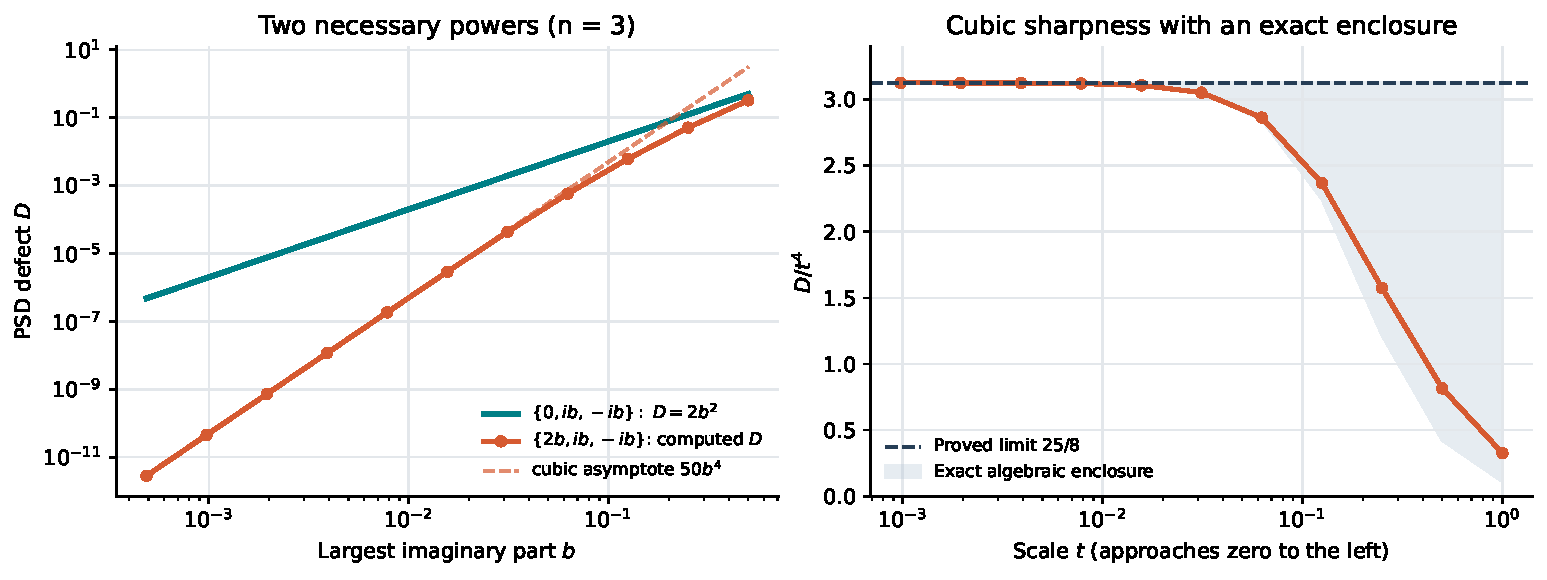
\includegraphics[width=0.94\textwidth]{figures/sharp_exponents.pdf}
\caption{For $n=3$, two exact root families exhibit the different limiting
powers. The cubic family has $\defect\sim50b^4$, while
$\{0,\I b,-\I b\}$ has $\defect=2b^2$. Numerical eigenvalues illustrate
identities and inequalities proved above; they are not used as proof.}
\label{fig:powers}
\end{figure}}{}

\section{Certified bounds with inaccurate moments}
\label{sec:noise}

Suppose real approximate moments $\widehat s_k$ come with proved errors
$|s_k-\widehat s_k|\leq e_k$, where $e_k\geq0$ for
$0\leq k\leq2n-2$. Define
\begin{equation}
 \widehat H=(\widehat s_{i+j})_{0\leq i,j<n},\qquad
 E=\min\left\{
 \max_i\sum_j e_{i+j},\;
 \left(\sum_{i,j}e_{i+j}^2\right)^{1/2}\right\}.
 \label{eq:errorbudget}
\end{equation}
The row-sum and Frobenius estimates both bound
$\|H-\widehat H\|_{\mathrm{op}}$, so their minimum is also valid.

\begin{corollary}[A two-sided certificate]
\label{cor:noise}
Under Theorem~\ref{thm:main}, suppose a certified interval
$[\ell,u]$ contains $\lambda_{\min}(\widehat H)$. Set
\[
 D_- =\max\{0,-u-E\},\qquad
 D_+ =\max\{0,-\ell+E\}.
\]
Then
\begin{equation}
 \sqrt{D_-/C_n}\leq b(Z)\leq
 \min\{1,K_n(D_+/2)^{1/(2n-2)}\}.
 \label{eq:certified}
\end{equation}
In particular, a certified $\widehat H\succeq-\tau I$, $\tau\geq0$,
gives
\begin{equation}
 b(Z)\leq\min\{1,K_n((\tau+E)/2)^{1/(2n-2)}\}.
 \label{eq:slack}
\end{equation}
If every $e_k\leq e$, one may use $E=ne$.
\end{corollary}

\begin{proof}
For every unit vector, the quadratic forms of $H$ and $\widehat H$ differ
by at most $E$. Minimizing over unit vectors bounds the smallest eigenvalue
of $H$ between $\ell-E$ and $u+E$, hence its defect between $D_-$ and
$D_+$. Apply \eqref{eq:inverse}.
\end{proof}

\begin{corollary}[Exact reality from a positive margin]
\label{cor:exact}
If $\widehat H\succeq\gamma I$ is certified with $\gamma>E$, then all
$n$ roots are real and distinct.
\end{corollary}
\begin{proof}
Then $H\succeq(\gamma-E)I\succ0$. Theorem~\ref{thm:main} gives reality.
If fewer than $n$ distinct locations occurred, the Vandermonde
factorization would make $H$ singular. Thus the roots are distinct.
\end{proof}

The required arithmetic certification can be elementary. For a rational
matrix, symmetric Schur elimination tests positive semidefiniteness exactly.
A negative pivot disproves it; a zero pivot requires the remaining row to be
zero; a positive pivot permits a Schur-complement step. For numerical
contour input, the errors $e_k$ must themselves come from rigorous bounds.
An unvalidated floating-point eigenvalue is not such a certificate.

As a concrete precision target, for $n=3$, $\tau=0$, and uniform error $e$,
\eqref{eq:slack} gives $b\leq4(3e/2)^{1/4}$. To certify $b\leq\eta$ by
this worst-case bound it suffices that
\begin{equation}
 e\leq\eta^4/384.
 \label{eq:precision}
\end{equation}
The constants are conservative, but the fourth power cannot be replaced by
a more favorable universal exponent for this certificate.

\section{Finite windows of zeta and Dirichlet zeros}
\label{sec:contour}

\subsection{The contour theorem}

\begin{theorem}[A local analytic certificate]
\label{thm:contour}
Let $\Omega$ be a bounded, conjugation-invariant domain contained in the
unit disk, with positively oriented piecewise smooth boundary $\Gamma$.
Let $F$ be holomorphic on a neighborhood of $\overline\Omega$, satisfy
$F(\overline z)=\overline{F(z)}$, and be nonzero on $\Gamma$.
Suppose $F$ has exactly $n\geq2$ zeros in $\Omega$, counted with
multiplicity. Define
\begin{equation}
 s_k=\frac1{2\pi\I}\int_\Gamma
 z^k\frac{F'(z)}{F(z)}\,dz,\qquad 0\leq k\leq2n-2.
 \label{eq:contour}
\end{equation}
Then these moments satisfy Theorem~\ref{thm:main} and
Corollary~\ref{cor:noise}, with $b$ equal to the largest imaginary part
in absolute value of a zero in $\Omega$.
\end{theorem}

\begin{proof}
The residue of $F'/F$ at a zero is its positive integer multiplicity.
The residue theorem turns \eqref{eq:contour} into \eqref{eq:hermite}.
The zeros in $\Omega$ are conjugation invariant, by the symmetry of both
$F$ and $\Omega$. Every zero lies in the unit disk. All hypotheses of the
finite-root result therefore hold.
\end{proof}

The contour representation and qualitative inertia test are prior work;
in the xi setting see Deng--Yang--L\"u \cite{deng}. The new application
here is the explicit error budget and sharp power in the resulting strip
estimate. The zero count must be established before selecting the matrix
size. For example, a certified error less than $1/2$ in $s_0$, together with
the zero-free boundary hypothesis, identifies its integer value by rounding.
If $n=0$, the window is empty; if $n=1$, conjugation symmetry already forces
its single zero to be real.

Holomorphy matters. For a meromorphic $F$ the contour moments would have
negative weights from poles, and Theorem~\ref{thm:main} would not apply
without first removing those poles.

\subsection{Riemann xi}

Use the classical entire function
\[
 \xi(s)=\frac12s(s-1)\pi^{-s/2}\Gamma(s/2)\zeta(s),
 \qquad \Xi(w)=\xi(1/2+\I w).
\]
The functional equation and conjugation identity imply that $\Xi$ is real
entire. Its zeros encode the nontrivial zeros of $\zeta$ \cite{dlmfzeta}.
For a real height $T$ and a scale $A>0$, set
$F(z)=\Xi(T+Az)$. A zero $z$ corresponds to
\begin{equation}
 \rho=\frac12+\I(T+Az),\qquad
 |\Repart\rho-1/2|=A|\Impart z|.
 \label{eq:coordinate}
\end{equation}
Consequently, if the normalized contour moments satisfy the certified
slack condition of \eqref{eq:slack}, every enclosed zero obeys
\begin{equation}
 \boxed{\quad
 |\Repart\rho-1/2|
 \leq A\min\{1,K_n((\tau+E)/2)^{1/(2n-2)}\}.
 \quad}
 \label{eq:zetastrip}
\end{equation}
No RH assumption was used in deriving this implication. RH supplies the
exact conclusion for the original xi function; the finite quantitative
statement is useful for audited numerical data and for other real-entire
functions or perturbations. It is not an additional global proof of RH.

\subsection{Primitive Dirichlet \texorpdfstring{$L$}{L}-functions}

Let $\chi$ be a primitive nonprincipal character of conductor $q$, with
$\chi(-1)=(-1)^a$, $a\in\{0,1\}$. The completed function
\[
 \Lambda_\chi(s)=
 (q/\pi)^{(s+a)/2}\Gamma((s+a)/2)L(s,\chi)
\]
is entire and has functional equation
\begin{equation}
 \Lambda_\chi(s)=\varepsilon_\chi\Lambda_{\overline\chi}(1-s),
 \qquad |\varepsilon_\chi|=1.
 \label{eq:dirfe}
\end{equation}
These standard facts and the Euler-factor distinction for imprimitive
characters are recorded in the DLMF \cite{dlmfdirichlet}.
Write $\varepsilon_\chi=e^{\I\theta}$ and define
\[
 F_\chi(z)=e^{-\I\theta/2}
 \Lambda_\chi(1/2+\I(T+Az)).
\]
This function is real entire, even when the character is complex. Indeed,
using $\overline{\Lambda_\chi(s)}=\Lambda_{\overline\chi}(\overline s)$
and \eqref{eq:dirfe} shows directly that
$\overline{F_\chi(z)}=F_\chi(\overline z)$.
Therefore \eqref{eq:zetastrip} holds with $\Lambda_\chi$ in place of
$\xi$. The phase cancels from $F_\chi'/F_\chi$, so computing contour
moments does not require choosing a numerical square root of the root number.

The primitive principal case is handled by $\xi$. An imprimitive character
should be reduced to its primitive completed function: the additional Euler
factors have their own zeros, and cannot silently be included in an assertion
that all zeros lie on the critical line. This is consistent with the Lean
repository's restriction to the open critical strip in its all-character
zero statement.

\section{Extensions and practical limits}

\subsection{A known bound on distinct locations}

If at most $d\geq2$ distinct root locations occur, the proof of
\eqref{eq:generalradius} improves the lower estimate, even when the matrix
has size $n>d$, to
\begin{equation}
 \defect(Z)\geq
 2\left(\frac{b(Z)}{4\floor{d/2}}\right)^{2d-2}.
 \label{eq:distinct}
\end{equation}
The all-degree sharpness examples have $n$ distinct points that coalesce as
$t$ tends to zero. Repetition itself does not force the worst exponent.

More generally, take $d\geq2$ distinct conjugation-invariant nodes in the unit
disk, with positive
weights invariant under conjugation, minimum weight $w_*>0$, and total
weight $W$. For their $d\times d$ power-sum matrix, the same proof gives
\[
 2w_*\left(\frac b{4\floor{d/2}}\right)^{2d-2}
 \leq\defect
 \leq\frac{W d(d-1)(7d-11)}6 b^2.
\]
The lower bound uses the two exterior weights, each at least $w_*$;
the upper bound replaces $n$ by $W$ in the Taylor sum.

\subsection{Scaling and matrix coordinates}

The numerical value of $\defect$ depends on the polynomial basis. Our
statement fixes the monomial basis and normalizes the root disk to radius
one. For a physical disk centered at height $T$ with scale $A$, one should
compute normalized moments directly as in \eqref{eq:coordinate}.
The matrix is not invariant under rescaling, and treating its smallest
eigenvalue as if it were a coordinate-free number would be incorrect.

For roots in $|z|\leq R$, \eqref{eq:generalradius} gives the lower
constant $2\floor{n/2}(1+R)$ instead of $K_n$. The upper constant becomes
\[
 \frac n2\max_{0\leq i<n}
 \sum_{\substack{0\leq j<n\\i+j\geq2}}
 (i+j)(i+j-1)R^{i+j-2}.
\]
Normalizing first is usually clearer.

\subsection{What this result does not establish}

The finite theorem does not establish a new prime-distribution estimate,
zero simplicity for all of xi, or GRH outside the Dirichlet setting. A finite
contour computation does not cover zeros outside that contour. Very large
$n$ gives a weak worst-case exponent and can make moment computation poorly
conditioned. Partitioning a range into smaller windows can improve the
bound if each new boundary and zero count is independently certified.

These limits do not affect the complete algebraic theorem. They identify
the information required for using it as a numerical or analytic certificate.

\section{Prior work, proposed novelty, and verification}

\subsection{What is established background}

The Hermite--Sylvester equivalence, the power-sum quadratic form, and
interpolation values $\I,-\I,0$ are classical. Nathanson explicitly gives
this interpolation proof \cite{nathanson}. Certified Hermite reconstruction
from approximate root coordinates was developed by Ayyildiz Akoglu and
Szanto \cite{akoglu,macis}. Bickel, Pascoe, and Sargent study Hankel-based
relaxations for entire-function zeros with a spacing condition
\cite{bickel}. Deng, Yang, and L\"u describe contour moments, local inertia,
and an RH positivity formulation \cite{deng}.

\begin{center}
\begin{tabularx}{\textwidth}{@{}>{\raggedright\arraybackslash}p{0.25\textwidth}>{\raggedright\arraybackslash}X@{}}
\toprule
Source & Relation to this note \\
\midrule
Nathanson & Supplies the qualitative interpolation mechanism. Our grouped
divided differences add a bound uniform over root collisions. \\
Ayyildiz Akoglu--Szanto & Certifies Hermite matrices from approximate roots.
Our implication goes from approximate positivity to a maximal imaginary height. \\
Bickel--Pascoe--Sargent & Studies inverse-power Hankel conditions for entire
functions with spacing. Our finite multiset result has no spacing assumption. \\
Deng--Yang--L\"u & Provides the local contour-moment and inertia setting.
Our stated addition is the explicit defect/error-to-strip bound. \\
\bottomrule
\end{tabularx}
\end{center}

\subsection{The precise originality claim}

The proposed contribution is the explicit comparison
\eqref{eq:main}, its collision-tolerant interpolation estimate, the
optimality proofs for both exponents, and the combined certified-error
statement \eqref{eq:certified}. The contour identity and the qualitative
RH reformulation are not claimed as new.

The targeted search examined the complete short Nathanson paper, relevant
sections of the multivariate certified-Hermite paper, and the setup and main
results of the Bickel--Pascoe--Sargent paper. The MACIS predecessor was
available only at abstract level. For the 2026 contour paper, the primary
indexed abstract was accessible but the full text could not be retrieved.
No matching sharp-exponent theorem was found in the sources checked.
This is a \emph{candidate original result with a complete proof}, not a
certified claim of historical priority. The remaining bibliographic work is
explicitly separated from the mathematical proof.

\subsection{Reproducible artifacts and evidence levels}

The archive contains this source and PDF, exact rational calculations,
high-precision illustrative eigenvalues, a figure, source provenance, and a
formalization roadmap. The Python program verifies the cubic matrix,
its Schur complement, the single-moment repair, and grouped interpolation
examples including repeated roots. It also checks exact rational positive
semidefiniteness. These are concrete checks of potentially error-prone
algebra; they do not replace the proofs for arbitrary $n$.

The eigenvalue table and plot are numerical illustrations. We do not present
them as certified computations of actual zeta zeros. The local xi and
Dirichlet results are proved conditional implications from explicitly
listed finite contour certificates; producing such a certificate for a
particular window requires validated quadrature and boundary nonvanishing.

The full theorem has not been formalized or compiled in Lean here. The
roadmap states the needed interfaces without adding unproved axioms to an
existing project. The archived source extracts from \repo{} are a partial
audit snapshot and retain their upstream license and notices; they are not
the full buildable GRH development.

\appendix
\section{A minimal certificate protocol}

For a proposed local zero calculation, the following data make the
conclusion in \eqref{eq:zetastrip} reviewable.
\begin{enumerate}
\item Specify $F$, $\Omega$, its zero-free boundary $\Gamma$, and the real
normalization parameters $T,A$. Prove holomorphy and conjugation symmetry.
\item Certify the integer zero count $n$. If $n\geq2$, obtain real
enclosures for moments of orders $0$ through $2n-2$.
\item Record rational centers $\widehat s_k$ and upper bounds $e_k$ for
their errors. Form $\widehat H$ and $E$ from \eqref{eq:errorbudget}.
\item Certify $\widehat H+\tau I\succeq0$ by an exact decomposition or
a rigorously bounded spectral calculation. Alternatively certify an
interval for its smallest eigenvalue.
\item Substitute in \eqref{eq:slack} or \eqref{eq:certified}, and multiply
by $A$ to recover horizontal distance in the $s$-plane.
\end{enumerate}
If the computed upper bound exceeds the radius, the correct conclusion
remains the trivial radius bound. If an error interval crosses zero, the
matrix's displayed decimal eigenvalue alone cannot settle its sign.

\clearpage

\begin{thebibliography}{99}
\addcontentsline{toc}{section}{References}
\small
\bibitem{readme} L. Sernau and collaborators, \emph{GRH for Dirichlet
$L$-functions, in Lean 4}, repository README and readable-edition README,
commit \texttt{72fead102f663d5c7a407964a13dc0cf9d977207}, 25 Nov. 2026.
\url{https://github.com/lsernau/grh-lean}.
\bibitem{statements} Same repository, \texttt{grh/src/Statements.lean},
at the commit above.
\url{https://github.com/lsernau/grh-lean/blob/72fead102f663d5c7a407964a13dc0cf9d977207/grh/src/Statements.lean}.
\bibitem{mainlean} Same repository, \texttt{grh/src/Main.lean}.
\bibitem{existence} Same repository,
\texttt{grh/src/New/Reduction/Data/Existence.lean}.
\bibitem{shortenough} Same repository,
\texttt{grh/src/New/Reduction/ShortAndEnough.lean}.
\bibitem{mainineq} Same repository,
\texttt{grh/src/New/Reduction/MainInequality.lean}.
\bibitem{onesided} Same repository,
\texttt{grh/src/New/Reduction/OneSidedBound.lean}.
\bibitem{primeerror} Same repository,
\texttt{grh/src/New/Reduction/Zeros/PrimeError.lean}.
\bibitem{criterion} Same repository,
\texttt{grh/src/New/Reduction/Zeros/Criterion.lean}.
\bibitem{landau} Same repository,
\texttt{grh/src/Lib/Analytic/Landau.lean}.
\bibitem{rubinstein} M. Rubinstein, \emph{Alp\"oge/Claude proof of the
Generalized Riemann Hypothesis}, verification records, accessed 26 Nov. 2026.
\url{https://www.math.uwaterloo.ca/~mrubinst/alpoge_claude_grh/}.
\bibitem{wiki} Wikipedia contributors, \emph{Riemann hypothesis},
retrieved 26 Nov. 2026. Used for context and source discovery.
\url{https://en.wikipedia.org/wiki/Riemann_hypothesis}.
\bibitem{nathanson} M. B. Nathanson, \emph{The Hermite--Sylvester criterion
for real-rooted polynomials}, Mathematical Gazette \textbf{105} (2021),
122--125; arXiv:1911.01745v2.
\url{https://arxiv.org/abs/1911.01745}.
\bibitem{akoglu} T. Ayyildiz Akoglu and A. Szanto,
\emph{Certified Hermite matrices from approximate roots}, Journal of Symbolic
Computation \textbf{117} (2023), 101--118;
\url{https://doi.org/10.1016/j.jsc.2022.12.001};
\url{https://arxiv.org/abs/2110.10313}.
\bibitem{macis} T. Ayyildiz Akoglu and A. Szanto,
\emph{Certified Hermite Matrices from Approximate Roots---Univariate Case},
MACIS 2019, Lecture Notes in Computer Science \textbf{11989} (2020), 3--9.
Publisher abstract inspected; full text not reviewed in this investigation.
\bibitem{bickel} K. Bickel, J. E. Pascoe, and M. Sargent,
\emph{Zero-free regions near a line}, Mathematische Zeitschrift
\textbf{305} (2023), article 39;
\url{https://doi.org/10.1007/s00209-023-03364-w};
\url{https://arxiv.org/abs/2108.04807}.
\bibitem{deng} Z. Deng, X. Yang, and H. L\"u,
\emph{Contour Hankel dynamics and indicator fields for the Riemann
$\Xi$-function}, arXiv:2608.11520 (2026).
\url{https://arxiv.org/abs/2608.11520}.
Primary indexed abstract inspected; full text inaccessible in this investigation.
\bibitem{dlmfzeta} NIST Digital Library of Mathematical Functions,
\S25.4, \emph{Reflection Formulas}, and \S25.10, \emph{Zeros}.
\url{https://dlmf.nist.gov/25.4}; \url{https://dlmf.nist.gov/25.10}.
\bibitem{dlmfdirichlet} NIST Digital Library of Mathematical Functions,
\S25.15, \emph{Dirichlet $L$-functions}.
\url{https://dlmf.nist.gov/25.15}.
\end{thebibliography}
\end{document}
